\documentclass[12pt,a4paper]{report}

%--------------------------------------------------
% Packages
%--------------------------------------------------

\usepackage[a4paper,margin=1in]{geometry}

\usepackage{graphicx}
\usepackage{float}
\usepackage{caption}
\usepackage{subcaption}
%\usepackage{booktabs}
\usepackage{array}
\usepackage{longtable}
\usepackage{multirow}
\usepackage{listings}
\usepackage{xcolor}
\usepackage{titlesec}
%\usepackage{setspace}
\usepackage{hyperref}
\usepackage{fancyhdr}
\usepackage{ragged2e}
%\usepackage{tocloft}


%\onehalfspacing

%--------------------------------------------------
% Hyperref
%--------------------------------------------------

\hypersetup{
colorlinks=true,
linkcolor=blue,
urlcolor=blue
}

%--------------------------------------------------
% Header/Footer
%--------------------------------------------------

\pagestyle{fancy}

\fancyhf{}

\fancyfoot[C]{\thepage}

%--------------------------------------------------
% Listings Style
%--------------------------------------------------

\lstset{
basicstyle=\ttfamily\small,
keywordstyle=\color{blue},
commentstyle=\color{green!60!black},
stringstyle=\color{red},
numbers=left,
numberstyle=\tiny,
stepnumber=1,
numbersep=8pt,
frame=single,
breaklines=true,
showstringspaces=false,
tabsize=2
}
%----------------------------------Custom Fotter
\fancypagestyle{githubpage}{
    \fancyhf{}
    \fancyfoot[L]{\small\href{https://github.com/kittusharma2553-design/2026_GIPEDI_KARUNA_SHARMA.git}{GitHub Repository}}
    \fancyfoot[R]{\thepage}
}
%--------------------------------------------------
% Document
%--------------------------------------------------

\begin{document}

%%%%%%%%%%%%%%%%%%%%%%%%%%%%%%%%%%%%%%%%%%%%%%%%%%%
%%%%%%%%%%%%%%%%%%%%%%%%%%%%%%%%%%%%%%%%%%%%%%%%%%%
% TITLE PAGE
%%%%%%%%%%%%%%%%%%%%%%%%%%%%%%%%%%%%%%%%%%%%%%%%%%%

\newgeometry{top=1in,bottom=1in,left=0.5in,right=0.5in}

\begin{titlepage}
\thispagestyle{empty}

\begin{center}

% Institute Name
\resizebox{\textwidth}{!}{%
\bfseries INDIAN INSTITUTE OF TECHNOLOGY DELHI}

\vspace{0.35cm}

{\Large New Delhi -- 110016}

\vspace{1cm}

% Logo

\includegraphics[width=0.22\textwidth]{IIT_Delhi_logo.png}

\vspace{1cm}

% Report Title
{\LARGE\bfseries GIPEDI INTERNSHIP REPORT}

\vspace{0.8cm}

Submitted in fulfillment of the requirements for the Internship Program

\vfill

\renewcommand{\arraystretch}{1.6}

\begin{tabular}{@{}ll@{}}

\textbf{Name:} &
Karuna Sharma \\

\textbf{Internship Period:} &
15 May 2026 -- 15 July 2026 \\

\textbf{Organization:} &
Department of Electrical Engineering \\
&
Indian Institute of Technology Delhi \\

\textbf{Supervisor:} &
Prof. Subrat Kar \\

\textbf{Mentor:} &
Mr. Utkarsh Roy \\

\end{tabular}

\vfill

{\Large July 2026}

\end{center}

\end{titlepage}

\restoregeometry

%%%%%%%%%%%%%%%%%%%%%%%%%%%%%%%%%%%%%%%%%%%%%%%%%%%
% Certifictae
%%%%%%%%%%%%%%%%%%%%%%%%%%%%%%%%%%%%%%%%%%%%%%%%%%%
\chapter*{Certificate}
\addcontentsline{toc}{chapter}{Certificate}

This is to certify that Ms. \textbf{Karuna Sharma} has successfully completed her internship work titled:

\begin{center}
\textbf{"GIPEDI INTERNSHIP REPORT"}
\end{center}

\begin{justify}
during the period from \textbf{15 May 2026 to 15 July 2026} under the guidance of \textbf{Prof. Subrat Kar}, Department of Electrical Engineering, Indian Institute of Technology Delhi.
\end{justify}
\begin{justify}
During the internship period, she worked sincerely and diligently on various experiments and projects related to embedded systems, electronics, and web application development. The work presented in this report is a record of the activities carried out during the internship period.
\end{justify}
\vspace{3cm}

\begin{flushleft}
\textbf{Prof. Subrat Kar}\\
Department of Electrical Engineering\\
Indian Institute of Technology Delhi
\end{flushleft}

\vspace{1cm}

\begin{flushright}
Date: \today
\end{flushright}

\newpage

%%%%%%%%%%%%%%%%%%%%%%%%%%%%%%%%%%%%%%%%%%%%%%%%%%%
% 
%%%%%%%%%%%%%%%%%%%%%%%%%%%%%%%%%%%%%%%%%%%%%%%%%%%
\chapter*{Acknowledgement}
\addcontentsline{toc}{chapter}{Acknowledgement}

I express my sincere gratitude to \textbf{Prof. Subrat Kar}, Department of Electrical Engineering, Indian Institute of Technology Delhi, for providing me with the opportunity to undertake this internship and for his valuable guidance and encouragement throughout the internship period.

\begin{justify}
I would also like to thank \textbf{Mr. Utkarsh Roy} for his continuous support, technical guidance, and valuable suggestions during the course of this work.
\end{justify}

\begin{justify}
I am grateful to the faculty members, staff, and colleagues of the Department of Electrical Engineering, IIT Delhi, for providing the necessary facilities and a conducive environment for learning and experimentation.
\end{justify}

Finally, I would like to thank everyone who directly or indirectly contributed to the successful completion of this internship.

\vspace{2cm}

\begin{flushright}
\textbf{Karuna Sharma}
\end{flushright}

\newpage
%%%%%%%%%%%%%%%%%%%%%%%%%%%%%%%%%%%%%%%%%%%%%%%%%%%
% TABLE OF CONTENTS
%%%%%%%%%%%%%%%%%%%%%%%%%%%%%%%%%%%%%%%%%%%%%%%%%%%

\tableofcontents

\newpage

%%%%%%%%%%%%%%%%%%%%%%%%%%%%%%%%%%%%%%%%%%%%%%%%%%%
% EXPERIMENT 0
%%%%%%%%%%%%%%%%%%%%%%%%%%%%%%%%%%%%%%%%%%%%%%%%%%%

\chapter{Arduino Basic Program}

\section {Objective}

\begin{itemize}

\item Learn the components of an Arduino Uno circuit.

\item Understand how to connect basic electronic components.

\item Write and upload a simple Arduino program.

\item Verify the circuit through simulation.

\end{itemize}

\section{Tools Required}

\begin{enumerate}

\item Arduino UNO 

\item LED

\item Arduino IDE

\end{enumerate}

\section{Circuit Diagram}

\begin{figure}[H]

\centering


\includegraphics[width=0.5\textwidth]{experiment0.png}

\caption{Arduino LED Blinking Circuit}

\end{figure}

\newpage

\section{Arduino Code}
The complete implementation code is available in the GitHub repository referenced in the footer.
% \begin{lstlisting}[language=C]

% const int ledPin = 9;

% void setup()
% {
%     pinMode(ledPin, OUTPUT);
% }

% void loop()
% {
%     digitalWrite(ledPin, HIGH);

%     delay(1000);

%     digitalWrite(ledPin, LOW);

%     delay(1000);
% }

% \end{lstlisting}

\section{Method}

The program repeatedly turns the LED ON for one second and OFF for one second, producing a continuous blinking effect.

\subsection{Learning Outcome}

\begin{itemize}

\item Learned how to connect an LED with Arduino Uno.

\item Learned to write and upload an Arduino program.

\item Understood basic digital output control.

\end{itemize}

\subsection{Problems Faced}

\subsubsection{Problem}

The LED did not blink after uploading the program.

%\vspace{0.3cm}

\subsubsection{Solution}

Checked the wiring connections and uploaded the program again.

\subsection{Future Scope}

\begin{itemize}

\item Control multiple LEDs.

\item Interface sensors with Arduino.

\item Develop simple automation projects.

\end{itemize}

\thispagestyle{githubpage}

%%%%%%%%%%%%%%%%%%%%%%%%%%%%%%%%%%%%%%%%%%%%%%%%%%%
% EXPERIMENT 1
%%%%%%%%%%%%%%%%%%%%%%%%%%%%%%%%%%%%%%%%%%%%%%%%%%%

\chapter{Experiment 1}

\section{Title}

Interface a Seven Segment LED Display Using a Push Button

\section{Objective}

To interface a seven-segment display with Arduino and use a push button to implement a counter.

\section{Tools Required}

\begin{enumerate}

\item Arduino UNO

\item Seven Segment Display (Common Cathode)

\item Push Button

\item Arduino IDE

\end{enumerate}

\section{Theory}

A seven-segment display consists of seven LEDs arranged in the shape of the number 8. By turning individual LEDs ON and OFF, digits from 0 to 9 can be displayed. A push button acts as the input device that increments the displayed count every time it is pressed.

\section{Circuit Diagram}

\begin{figure}[H]

\centering

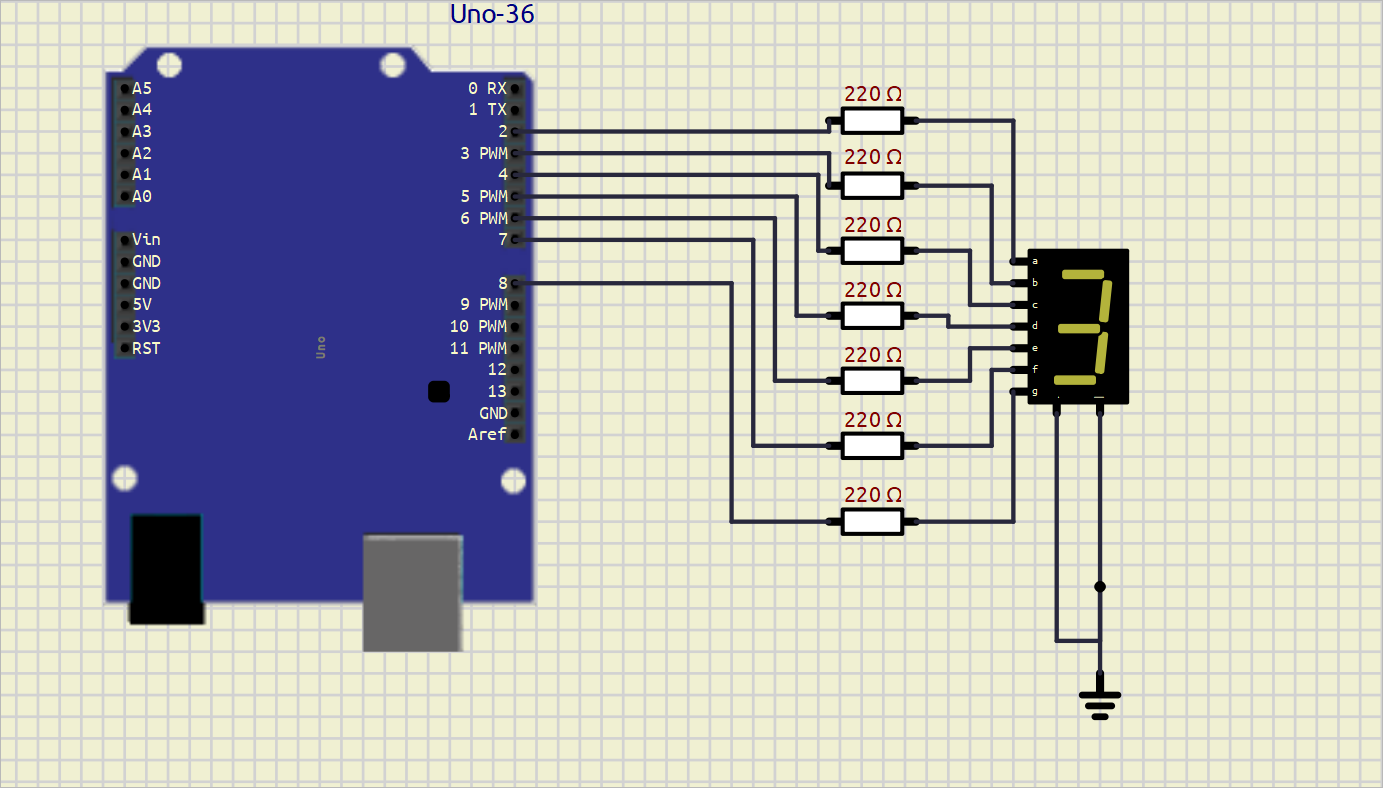
\includegraphics[width=0.35\textwidth]{7-Segment.png}

\caption{Interfacing Seven Segment Display with Arduino}

\end{figure}



%%%%%%%%%%%%%%%%%%%%%%%%%%%%%%%%%%%%%%%%%%%%%%%%%%%
% EXPERIMENT 1 (Continued)
%%%%%%%%%%%%%%%%%%%%%%%%%%%%%%%%%%%%%%%%%%%%%%%%%%%

\subsection{Arduino Code}
The complete implementation code is available in the GitHub repository referenced in the footer.

\section{Procedure}

\begin{enumerate}

\item Connect the seven-segment display to the Arduino digital pins.

\item Connect the push button to the Arduino input pin.

\item Upload the program using the Arduino IDE.

\item Press the push button repeatedly.

\item Observe the number displayed on the seven-segment display.

\end{enumerate}

\section{Observations}

\begin{itemize}

\item The display initially shows 0.

\item Each button press increments the displayed number.

\item After reaching 9, the counter resets to 0.

\end{itemize}

\section{Learning Outcome}

\begin{itemize}

\item Learned to interface a seven-segment display with Arduino.

\item Digital input was detected using a push button.

\item Implemented a simple counter using Arduino.

\end{itemize}

\thispagestyle{githubpage}


\section{Problems Faced}

\subsubsection{Problem}

Incorrect digits were displayed on the seven-segment display due to incorrect wiring.

\vspace{0.1cm}

\subsubsection{Solution}

The segment pin connections were checked and corrected according to the circuit diagram, after which the display operated correctly.

\section{Future Scope}

\begin{itemize}

\item Four-digit digital counters.

\item Visitor counting systems.

\item Digital scoreboards.

\item Electronic voting and counting systems.

\end{itemize}

%%%%%%%%%%%%%%%%%%%%%%%%%%%%%%%%%%%%%%%%%%%%%%%%%%%
% EXPERIMENT 2
%%%%%%%%%%%%%%%%%%%%%%%%%%%%%%%%%%%%%%%%%%%%%%%%%%%

\chapter{Experiment 2}

\section{Title}

Display Different Patterns on an LED Matrix

\section{Objective}

To interface an LED matrix with Arduino Uno and display different patterns, symbols, and designs.

\section{Tools Required}

\begin{enumerate}

\item Arduino Uno

\item 8×8 LED Matrix

\item Arduino IDE

\end{enumerate}

\section{Theory}

An LED matrix is a collection of LEDs arranged in rows and columns. By controlling each LED individually, different symbols, letters, numbers, patterns, and animations can be displayed. Arduino sends binary data to illuminate selected LEDs and generate the desired output.

\section{Circuit Diagram}

\begin{figure}[H]

\centering

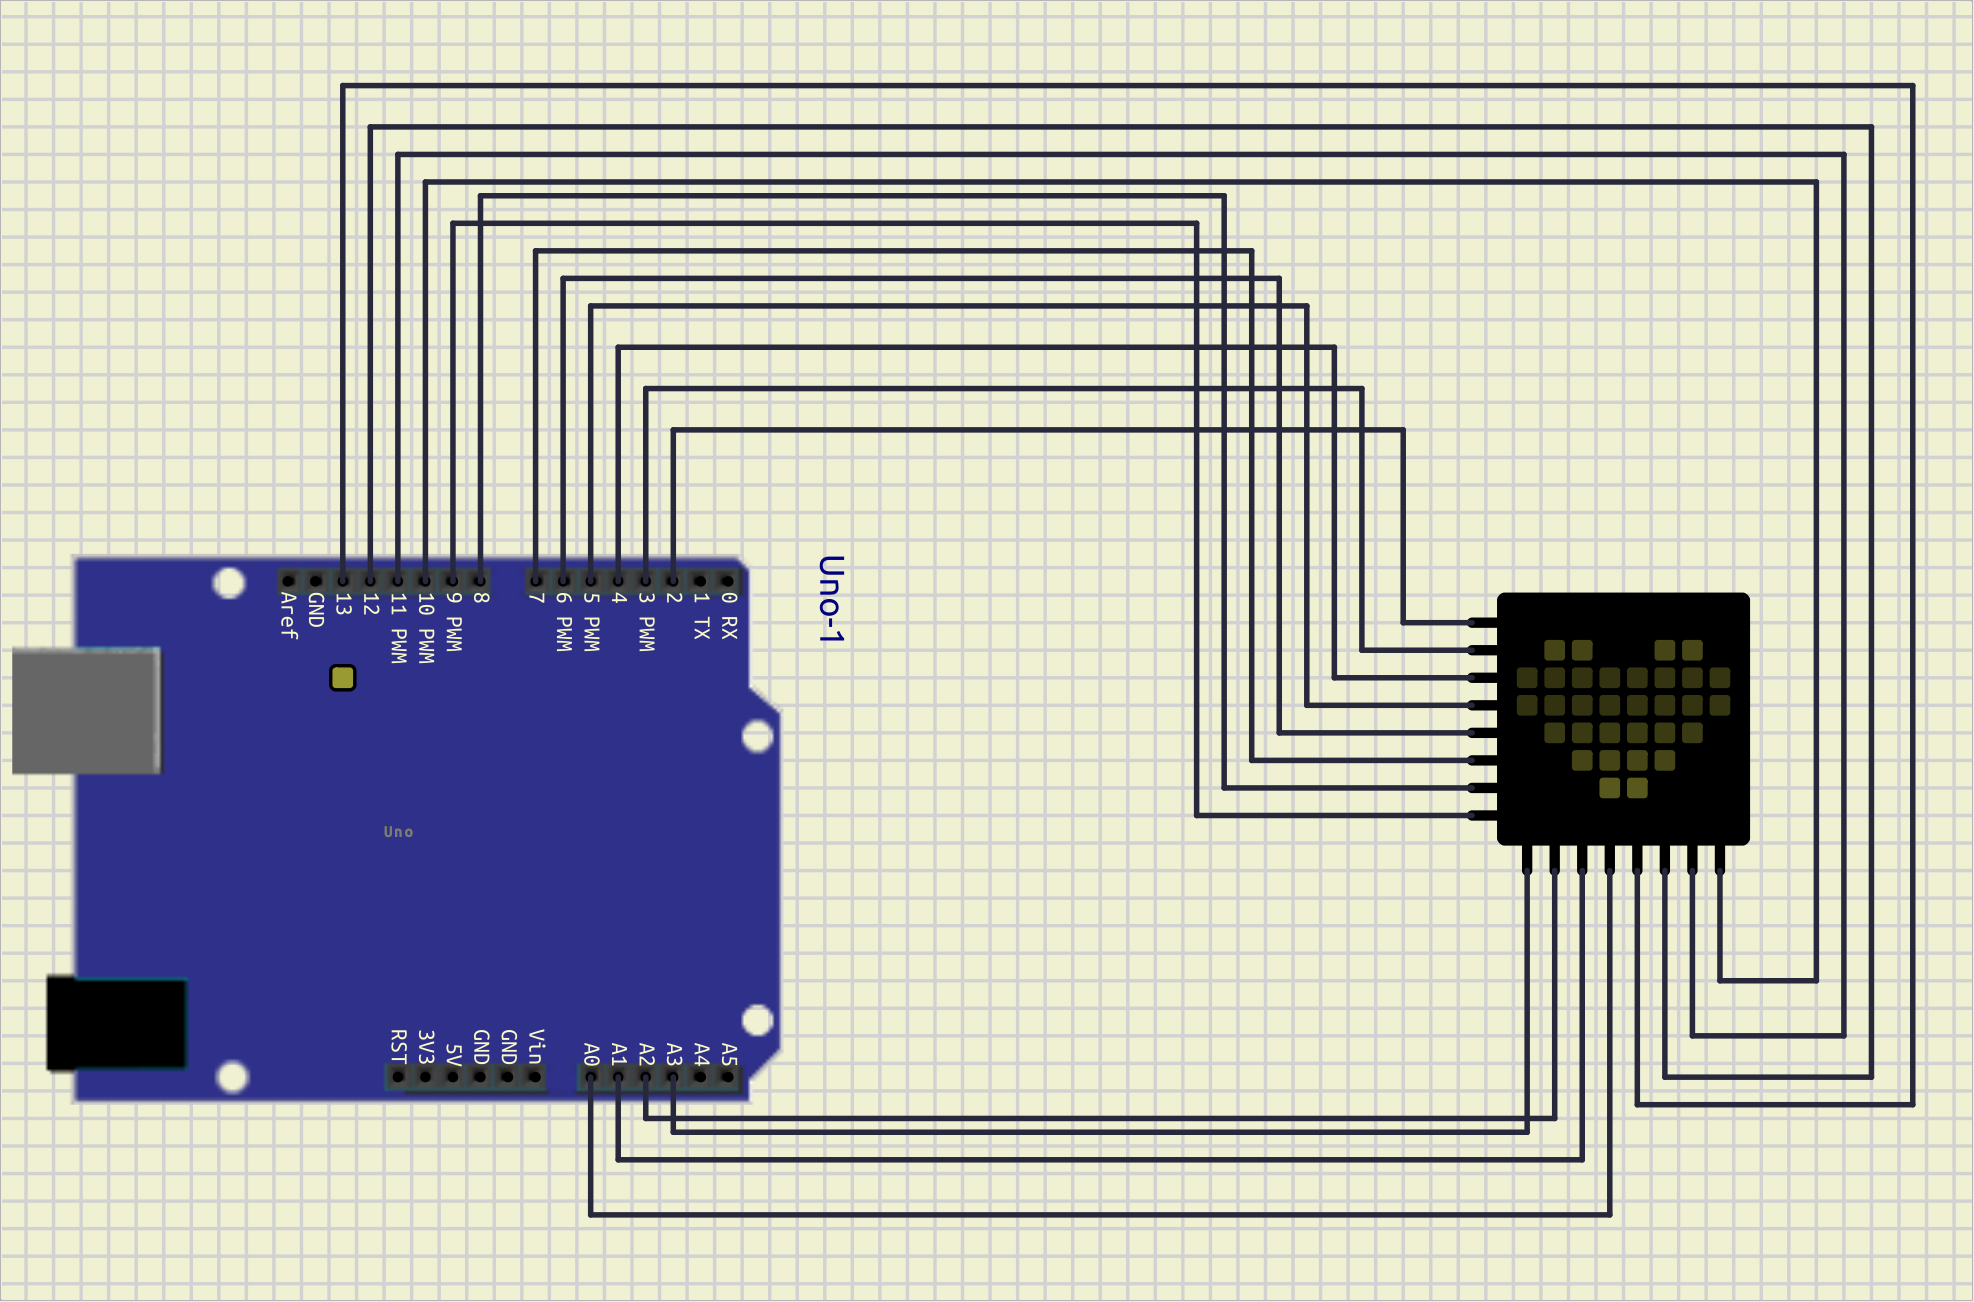
\includegraphics[width=0.35\textwidth]{experiment3.png
}

\caption{Interfacing an LED Matrix with Arduino Uno}

\end{figure}

\section{Arduino Code}

The complete implementation code is available in the GitHub repository referenced in the footer.

\thispagestyle{githubpage} %-----This is For Fotter-----%
 

% \begin{lstlisting}[language=C++]
% int pins[] =
% {
% 2,3,4,5,6,7,
% 8,9,10,11,12,13
% };

% void setup()
% {
%     for(int i=0;i<12;i++)
%     {
%         pinMode(pins[i],OUTPUT);
%     }
% }

% void loop()
% {
%     for(int i=0;i<12;i++)
%     {
%         digitalWrite(pins[i],HIGH);
%     }

%     delay(1000);

%     for(int i=0;i<12;i++)
%     {
%         digitalWrite(pins[i],LOW);
%     }

%     delay(1000);
% }
%\end{lstlisting}


\section{Procedure}

\begin{enumerate}

\item Connect the LED matrix to the Arduino.

\item Upload the program using the Arduino IDE.

\item Run the circuit.

\item Observe the displayed pattern.

\item Modify the binary data to display different symbols and designs.

\end{enumerate}

\section{Observations}

\begin{itemize}

\item The LED matrix successfully displayed the programmed pattern.

\item Different patterns were obtained by changing the binary values.

\item Letters, numbers, symbols, and simple animations can be displayed.

\end{itemize}

\section{Learning Outcome}

\begin{itemize}

\item Learned how to interface an LED matrix with Arduino.

\item Understood row and column addressing.

\item Gained experience in creating visual patterns using programming.

\end{itemize}

\section{Problems Faced}

\subsubsection{Problem}

The LED matrix did not display the correct pattern.

\vspace{0.3cm}

\subsubsection{Solution}

Checked all wiring connections and verified the binary pattern data in the program.

\section{Future Scope}

\begin{itemize}

\item Scrolling text displays.

\item Animation systems.

\item LED notice boards.

\item Electronic display systems.

\end{itemize}

\newpage

%%%%%%%%%%%%%%%%%%%%%%%%%%%%%%%%%%%%%%%%%%%%%%%%%%%
% NEXT CHAPTER:
% PROJECT ON 555 TIMER IC
%%%%%%%%%%%%%%%%%%%%%%%%%%%%%%%%%%%%%%%%%%%%%%%%%%%

%%%%%%%%%%%%%%%%%%%%%%%%%%%%%%%%%%%%%%%%%%%%%%%%%%%
% PROJECT ON 555 TIMER IC
%%%%%%%%%%%%%%%%%%%%%%%%%%%%%%%%%%%%%%%%%%%%%%%%%%%

\chapter{Project on 555 Timer IC}

\section{Title}

Design and Implementation of a 555 Timer Circuit

\section{Aim}

To study the working of the 555 Timer IC and generate timing pulses using an astable multivibrator circuit.

\section{Objectives}

\begin{enumerate}
    \item To understand the operation of the 555 Timer IC.
    \item To generate a continuous square-wave output.
    \item To observe the charging and discharging characteristics of a capacitor.
\end{enumerate}

\section{Components Required}

\begin{enumerate}
    \item NE555 Timer IC
    \item Resistor R1 (1 k$\Omega$)
    \item Resistor R2 (10 k$\Omega$)
    \item Capacitor C1 (10 $\mu$F)
    \item Breadboard
    \item Connecting wires
    \item 5 V DC Power Supply
    \item LED
\end{enumerate}

\section{Circuit Diagram}

\begin{figure}[H]
\centering

\includegraphics[width=0.45\textwidth]{ne555_timer.png}
\caption{Astable Multivibrator using NE555 Timer IC}
\end{figure}

\begin{figure}[H]
\centering
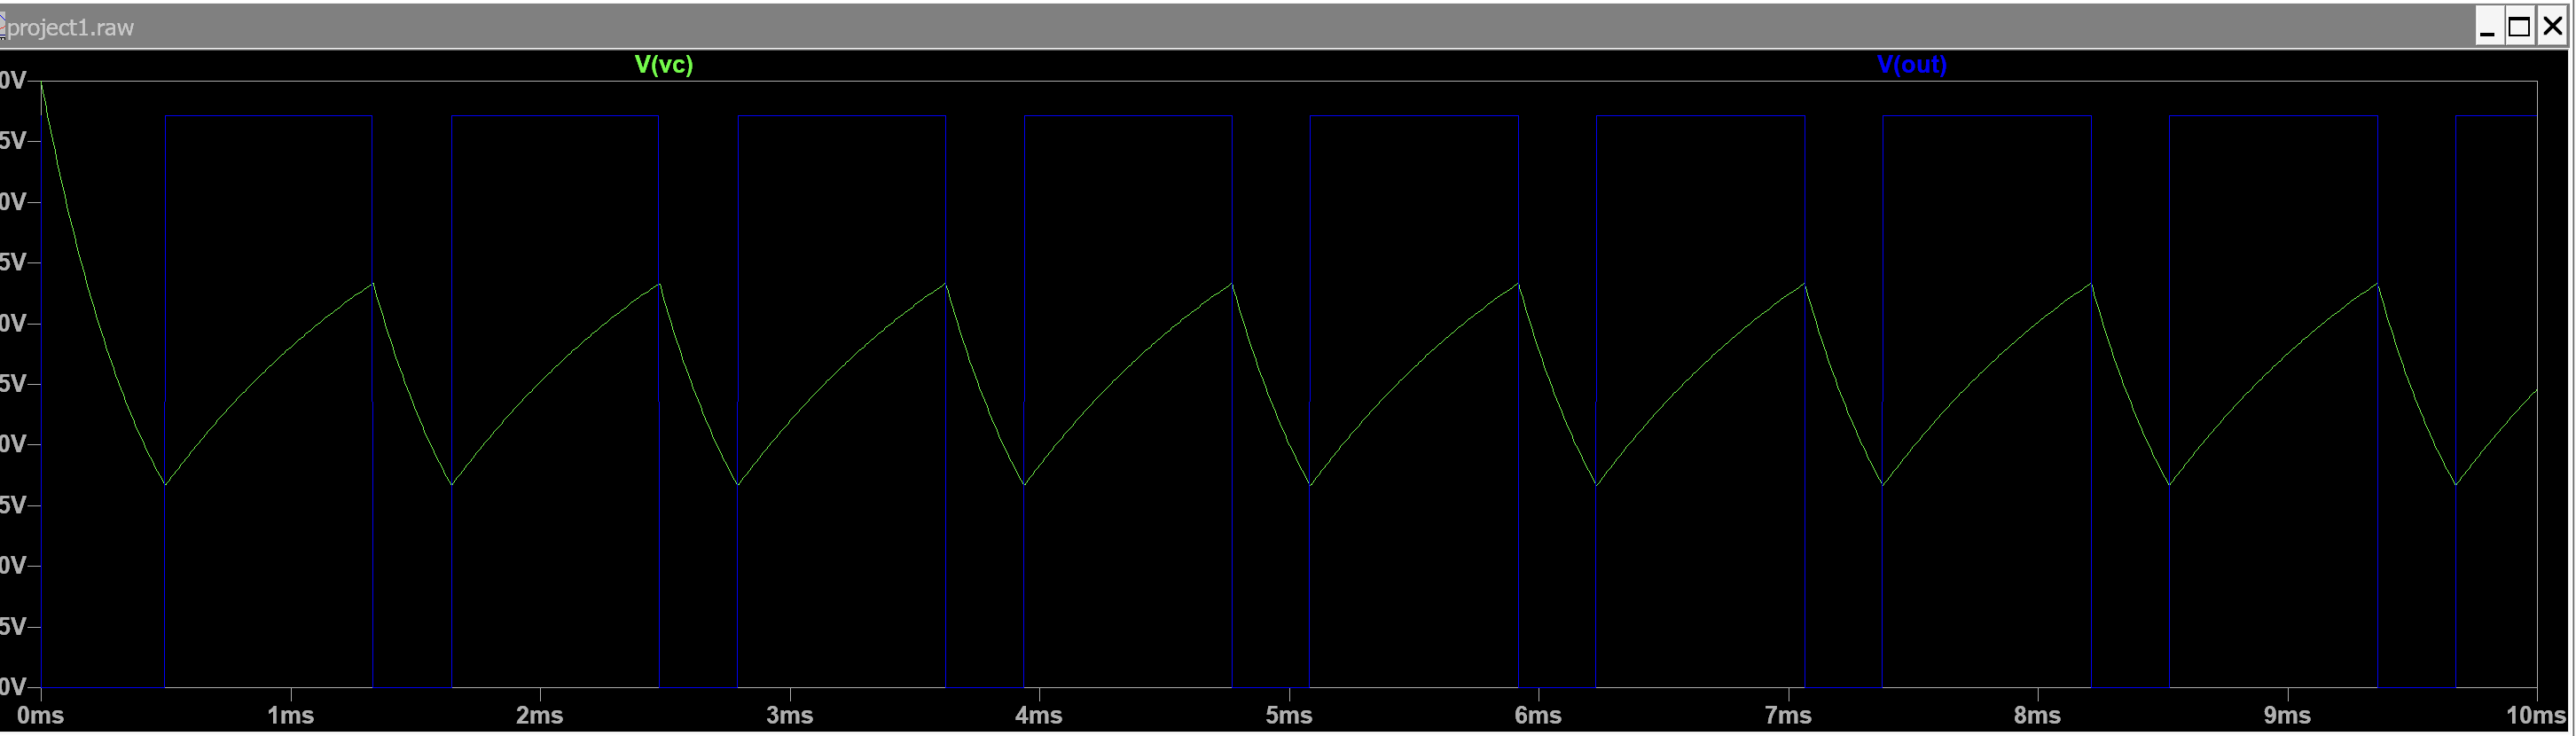
\includegraphics[width=0.85\textwidth]{project on 555timer ic output.png}
\caption{Output Waveform}
\end{figure}

\section{Theory}

The NE555 Timer is one of the most widely used integrated circuits in electronic applications. It can operate in three modes:

\begin{itemize}
\item Astable Mode
\item Monostable Mode
\item Bistable Mode
\end{itemize}

In this experiment, the IC operates in astable mode, where the output continuously switches between HIGH and LOW without requiring an external trigger.

The charging and discharging of capacitor C1 through resistors R1 and R2 determines the output frequency.

\section{Procedure}

\begin{enumerate}

\item Place the NE555 IC on the breadboard.

\item Connect the circuit according to the circuit diagram.

\item Connect the LED at the output pin through a resistor.

\item Apply a 5 V power supply.

\item Observe the blinking LED.

\item Measure the output waveform if an oscilloscope is available.

\end{enumerate}

\section{Observations}

\begin{itemize}

\item The LED blinked continuously.

\item The blinking frequency depended upon the resistor and capacitor values.

\item A square-wave output was obtained at the output pin.

\item Changing capacitor values changed the blinking speed.

\end{itemize}

\section{Applications}

\begin{itemize}

\item LED Flashers

\item Pulse Generators

\item Clock Circuits

\item Alarm Systems

\item Tone Generators

\item PWM Circuits

\end{itemize}

\section{Advantages}

\begin{itemize}

\item Low cost

\item Simple circuit

\item Highly reliable

\item Easy to design

\item Wide operating voltage range

\end{itemize}

\section{Conclusion}

The project successfully demonstrated the working principle of the NE555 Timer IC in astable mode. The circuit generated periodic square-wave pulses, illustrating how resistor and capacitor values determine the output frequency.

\newpage

%%%%%%%%%%%%%%%%%%%%%%%%%%%%%%%%%%%%%%%%%%%%%%%%%%%
% OP AMP
%%%%%%%%%%%%%%%%%%%%%%%%%%%%%%%%%%%%%%%%%%%%%%%%%%%

\chapter{Inverting and Non-Inverting Amplifier using Operational Amplifier}

\section{Aim}

To study and analyze the operation of inverting and non-inverting amplifiers using an Operational Amplifier.

\section{Objectives}

\begin{enumerate}

\item To understand the working principle of inverting and non-inverting amplifiers.

\item To calculate and verify the voltage gain.

\item To compare their characteristics.

\item To study practical applications.

\end{enumerate}

\section{Components Required}

\begin{enumerate}

\item IC 741 Operational Amplifier

\item Breadboard

\item DC Power Supply

\item Resistors

\item Connecting Wires

\item Function Generator

\item Digital Multimeter

\item Oscilloscope

\end{enumerate}

\section{Theory}

An Operational Amplifier (Op-Amp) is a high-gain differential amplifier used in analog electronic circuits.

An inverting amplifier produces an output that is 180$^\circ$ out of phase with the input signal.

A non-inverting amplifier produces an amplified output while maintaining the same phase as the input signal.

The voltage gain of an inverting amplifier is

\[
A_v=-\frac{R_f}{R_{in}}
\]

where

\begin{itemize}

\item $R_f$ = Feedback Resistance

\item $R_{in}$ = Input Resistance

\end{itemize}

The voltage gain of a non-inverting amplifier is

\[
A_v=1+\frac{R_f}{R_1}
\]

\section{Circuit Diagrams}

\begin{figure}[H]
\centering

\begin{subfigure}{0.48\textwidth}
    \centering
    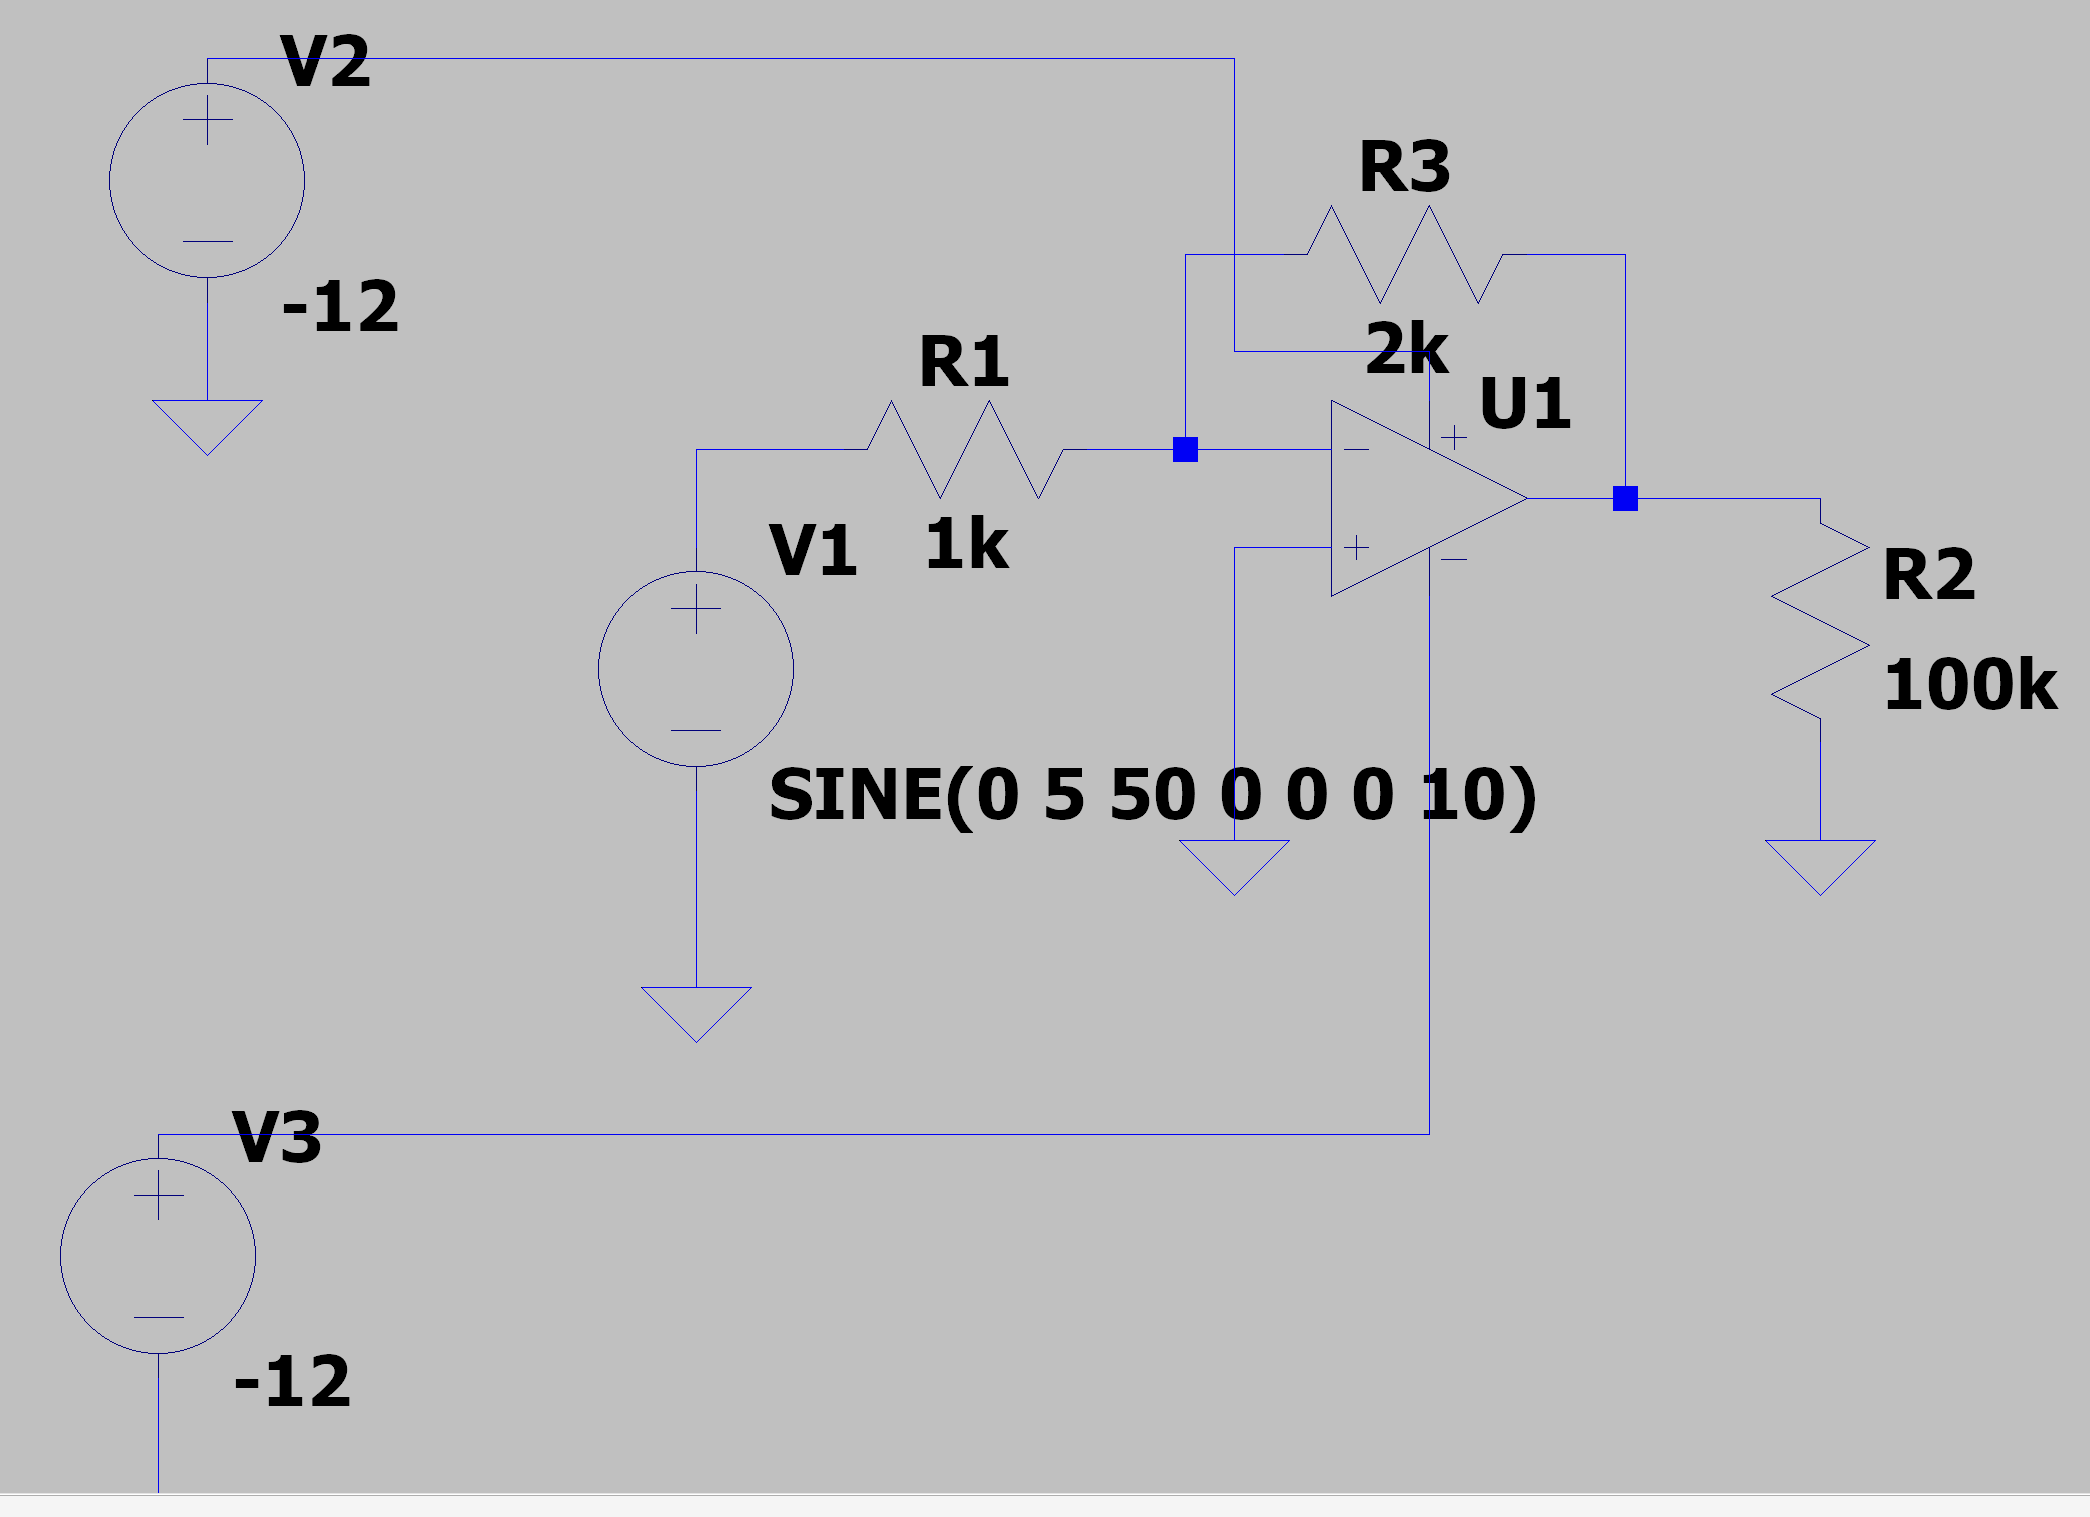
\includegraphics[height=5cm]{second_2.png}
    \caption{Non-Inverting Amplifier}
\end{subfigure}
\hfill
\begin{subfigure}{0.48\textwidth}
    \centering
    
\includegraphics[height=5cm]{3diagram.png}
    \caption{Inverting Amplifier}
\end{subfigure}

\end{figure}

\begin{figure}[H]
\centering
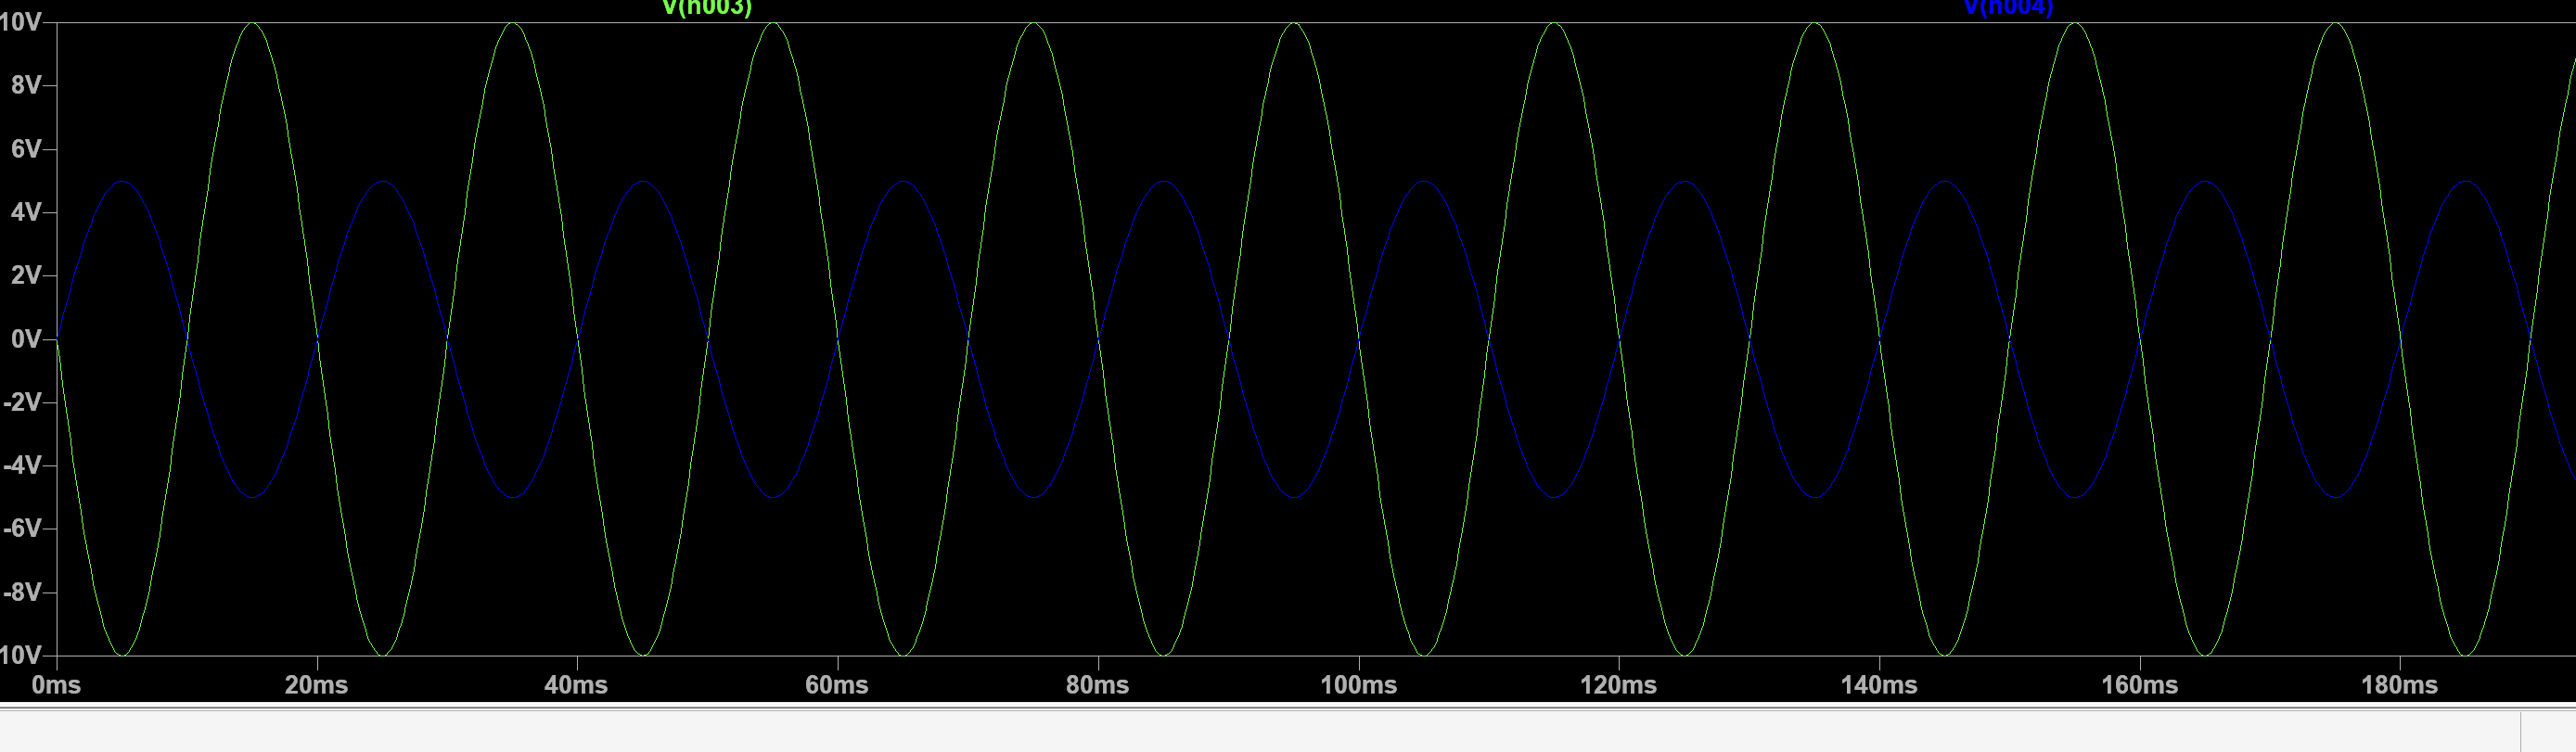
\includegraphics[width=0.85\textwidth]{inverting andnon inverting amplifier output.png}
\caption{Output Waveform}
\end{figure}



\section{Procedure}

\begin{enumerate}

\item Assemble the inverting amplifier circuit.

\item Apply a sinusoidal input signal.

\item Observe the output waveform.

\item Measure the voltage gain.

\item Repeat the same procedure for the non-inverting amplifier.

\item Compare the results.

\end{enumerate}

\section{Observations}

\begin{itemize}

\item The inverting amplifier output was 180$^\circ$ out of phase.

\item The non-inverting amplifier output remained in phase.

\item The measured gain closely matched the theoretical value.

\item The output remained stable throughout the experiment.

\end{itemize}

\section{Applications}

\subsection*{Inverting Amplifier}

\begin{itemize}

\item Signal Conditioning

\item Audio Amplifiers

\item Active Filters

\item Analog Computing

\end{itemize}

\subsection*{Non-Inverting Amplifier}

\begin{itemize}

\item Voltage Followers

\item Sensor Signal Amplification

\item Instrumentation Circuits

\item Buffer Amplifiers

\end{itemize}

\section{Advantages}

\begin{itemize}

\item High input impedance

\item Stable voltage gain

\item Excellent linearity

\item Low distortion

\item Easy implementation

\end{itemize}

\section{Conclusion}

The experiment verified the working of both inverting and non-inverting Operational Amplifier configurations. The measured voltage gain closely matched theoretical calculations, demonstrating the effectiveness of Operational Amplifiers in signal amplification.

\newpage

%%%%%%%%%%%%%%%%%%%%%%%%%%%%%%%%%%%%%%%%%%%%%%%%%%%
% NEXT CHAPTER
%%%%%%%%%%%%%%%%%%%%%%%%%%%%%%%%%%%%%%%%%%%%%%%%%%%

% Typing Progress Report

%%%%%%%%%%%%%%%%%%%%%%%%%%%%%%%%%%%%%%%%%%%%%%%%%%%
% CHAPTER : TYPING PROGRESS REPORT
%%%%%%%%%%%%%%%%%%%%%%%%%%%%%%%%%%%%%%%%%%%%%%%%%%%

\chapter{Typing Progress Report}

\section{Objective}

To improve typing speed and accuracy through daily practice and monitor the progress throughout the internship period.

\section{Typing Performance}

\begin{table}[H]
\centering
\caption{Typing Progress Report}

\begin{minipage}{0.48\textwidth}
\centering
\footnotesize
\begin{tabular}{|c|c|c|}
\hline
\textbf{S. No.} & \textbf{Date} & \textbf{WPM} \\
\hline
1 & 02/06/2026 & 24\\
2 & 03/06/2026 & 24\\
3 & 04/06/2026 & 24\\
4 & 05/06/2026 & 22\\
5 & 06/06/2026 & 23\\
6 & 07/06/2026 & 26\\
7 & 08/06/2026 & 30\\
8 & 09/06/2026 & 30\\
9 & 10/06/2026 & 28\\
10 & 11/06/2026 & 23\\
11 & 12/06/2026 & 26\\
12 & 13/06/2026 & 27\\
13 & 14/06/2026 & 27\\
14 & 15/06/2026 & 26\\
15 & 16/06/2026 & 26\\
16 & 17/06/2026 & 25\\
17 & 18/06/2026 & 26\\
18 & 19/06/2026 & 25\\
\hline
\end{tabular}
\end{minipage}
\hfill
\begin{minipage}{0.48\textwidth}
\centering
\footnotesize
\begin{tabular}{|c|c|c|}
\hline
\textbf{S. No.} & \textbf{Date} & \textbf{WPM} \\
\hline
19 & 20/06/2026 & 26\\
20 & 21/06/2026 & 27\\
21 & 22/06/2026 & 27\\
22 & 23/06/2026 & 26\\
23 & 24/06/2026 & 26\\
24 & 25/06/2026 & 25\\
25 & 26/06/2026 & 26\\
26 & 27/06/2026 & 25\\
27 & 28/06/2026 & 27\\
28 & 29/06/2026 & 27\\
29 & 30/06/2026 & 30\\
30 & 01/07/2026 & 30\\
31 & 02/07/2026 & 29\\
32 & 03/07/2026 & 30\\
33 & 04/07/2026 & 27\\
34 & 05/07/2026 & 29\\
35 & 06/07/2026 & 29\\
36 & 07/07/2026 & 30\\
\hline
\end{tabular}
\end{minipage}

\end{table}

\section{Typing Progress Graph}

\begin{figure}[H]
\centering
\fbox{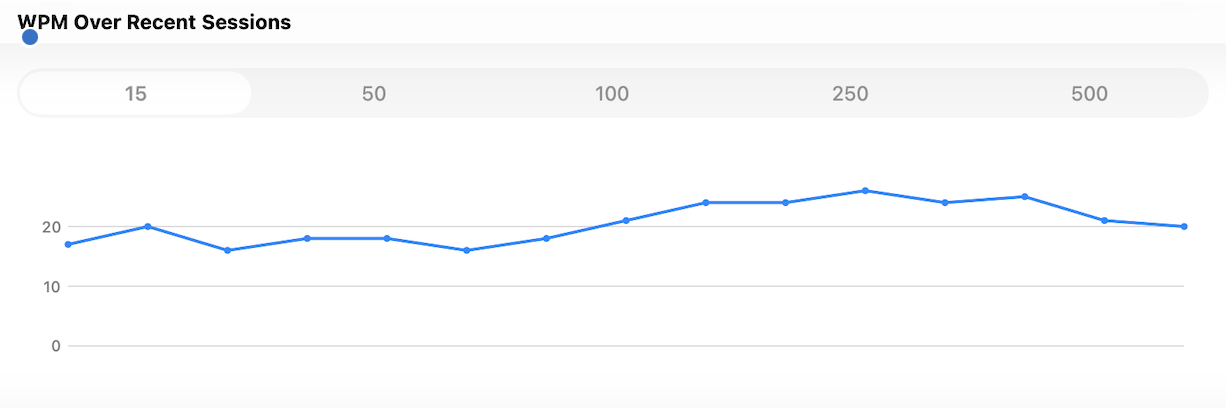
\includegraphics[width=0.65\textwidth]{typing report graph.png}}
\caption{Typing Progress Graph}
\end{figure}

\section{Observation}

\begin{itemize}
\item Daily typing practice improved typing speed.
\item Typing speed gradually increased from 22--24 WPM to approximately 30 WPM.
\item Accuracy and consistency also improved during the internship.
\end{itemize}

\section{Conclusion}

Regular typing practice significantly improved typing speed, accuracy, and keyboard familiarity, which are essential skills for technical documentation and programming.


%%%%%%%%%%%%%%%%%%%%%%%%%%%%%%%%%%%%%%%%%%%%%%%%%%%
% HTML WITH SQL DATABASE
%%%%%%%%%%%%%%%%%%%%%%%%%%%%%%%%%%%%%%%%%%%%%%%%%%%

\chapter{HTML with MySQL Database}

\section{Aim}

To develop a simple web application using HTML and store user information in an SQL database.

\section{Objectives}

\begin{enumerate}
\item Design a user input form using HTML.
\item Store the entered data in a MySQL database.
\item Retrieve and display records from the database.
\end{enumerate}

\section{Software Required}

\begin{enumerate}
\item Notepad++
\item XAMPP Server
\item MySQL Database
\item PHP
\item Web Browser
\end{enumerate}

\section{Hardware Requirements}

\begin{enumerate}
\item Desktop or Laptop Computer
\item Minimum 4 GB RAM
\item 500 MB Free Disk Space
\end{enumerate}

\section{Introduction}

HTML (HyperText Markup Language) is used to create web pages and collect user information through forms. Since HTML cannot communicate directly with a database, a server-side scripting language such as PHP is used to process the submitted form data and interact with a MySQL database.

This project demonstrates a simple student registration system in which user details entered through an HTML form are stored in a MySQL database.

\section{Theory}

\subsection*{HTML}

HTML provides the basic structure of a web page and allows developers to create forms, buttons, labels, and text fields for user interaction.

\subsection*{SQL}

Structured Query Language (SQL) is used to create, manage, update, and retrieve information from relational databases.

\subsection*{PHP}

PHP acts as an intermediary between HTML and MySQL. It receives the submitted form data and executes SQL queries to store or retrieve information.

\section{Flow of the System}

\begin{enumerate}
\item User opens the registration page.
\item User enters personal details.
\item Form data is submitted to a PHP script.
\item PHP establishes a connection with MySQL.
\item SQL query inserts the data into the database.
\item A success message is displayed to the user.
\end{enumerate}

\section{SQL Database}

\begin{figure}[H]
\centering
\fbox{\includegraphics[width=0.65\textwidth]{STUDENT_MARKs.png}}
\caption{Student Marks Database Table}
\end{figure}

%%%%%%%%%%%%%%%%%%%%%%%%%%%%%%%%%%%%%%%%%%%%%%%%%%%
% NEXT CONTINUATION
%%%%%%%%%%%%%%%%%%%%%%%%%%%%%%%%%%%%%%%%%%%%%%%%%%%

% HTML Source Code

%%%%%%%%%%%%%%%%%%%%%%%%%%%%%%%%%%%%%%%%%%%%%%%%%%%
% HTML SOURCE CODE
%%%%%%%%%%%%%%%%%%%%%%%%%%%%%%%%%%%%%%%%%%%%%%%%%%%

\section{HTML Source Code}
The complete HTML source code for this project is available in the GitHub repository linked in the footer.

\thispagestyle{githubpage}

% \begin{lstlisting}[language=HTML]
% <!DOCTYPE html>
% <html lang="en">

% <head>

% <meta charset="UTF-8">

% <meta name="viewport"
% content="width=device-width, initial-scale=1.0">

% <title>Student Registration</title>

% <style>

% body{
% font-family:Arial,sans-serif;
% background:#f4f4f4;
% text-align:center;
% margin-top:40px;
% }

% .container{

% width:400px;
% margin:auto;
% background:white;
% padding:20px;
% border-radius:8px;

% box-shadow:0 0 10px rgba(0,0,0,.2);

% }

% input{

% width:90%;
% padding:10px;
% margin:8px;

% }

% button{

% padding:10px 20px;
% background:#4CAF50;
% color:white;
% border:none;
% cursor:pointer;

% }

% button:hover{

% background:#45a049;

% }

% </style>

% </head>

% <body>

% <div class="container">

% <h2>Student Registration Form</h2>

% <form action="insert.php" method="POST">

% <input
% type="text"
% name="name"
% placeholder="Student Name"
% required>

% <input
% type="text"
% name="roll"
% placeholder="Roll Number"
% required>

% <input
% type="email"
% name="email"
% placeholder="Email Address"
% required>

% <input
% type="submit"
% value="Submit">

% </form>

% </div>

% </body>

% </html>

% \end{lstlisting}

%%%%%%%%%%%%%%%%%%%%%%%%%%%%%%%%%%%%%%%%%%%%%%%%%%%

\section{Advantages}

\begin{itemize}

\item Easy data management.

\item Reduces paperwork.

\item Fast data retrieval.

\item Improves efficiency.

\item Better data accuracy.

\end{itemize}

%%%%%%%%%%%%%%%%%%%%%%%%%%%%%%%%%%%%%%%%%%%%%%%%%%%

\section{Applications}

\begin{itemize}

\item Student Management Systems

\item College Record Systems

\item Employee Management

\item Library Management Systems

\item Hospital Registration Systems

\end{itemize}

%%%%%%%%%%%%%%%%%%%%%%%%%%%%%%%%%%%%%%%%%%%%%%%%%%%

\section{Output}

The user enters details into the HTML form. The information is transferred to a PHP script and stored successfully in the MySQL database.

%%%%%%%%%%%%%%%%%%%%%%%%%%%%%%%%%%%%%%%%%%%%%%%%%%%

\section{Conclusion}

This project demonstrated how HTML can be used to collect user information and how PHP and MySQL work together to store and retrieve data efficiently. The experiment provided practical knowledge of front-end and back-end web development.

\newpage

%%%%%%%%%%%%%%%%%%%%%%%%%%%%%%%%%%%%%%%%%%%%%%%%%%%
% NEXT CHAPTER
%%%%%%%%%%%%%%%%%%%%%%%%%%%%%%%%%%%%%%%%%%%%%%%%%%%

\chapter{Dashboard Button Interface}

\section{Aim}

To study the operation of button controls in a Battery Management System (BMS) graphical user interface.

\section{Objective}

To understand how button controls interact with software components for monitoring and controlling battery parameters.

\section{Theory}

A Button Control is a Graphical User Interface (GUI) component that executes an assigned action whenever it is clicked.

In Battery Management Systems, button controls are commonly used to

\begin{itemize}

\item Display battery information.

\item Select battery cells.

\item Monitor voltage.

\item View temperature.

\item Display charging status.

\end{itemize}

\section{Software Required}

\begin{enumerate}

\item HTML

\item CSS

\item JavaScript

\item Visual Studio Code

\item Web Browser

\end{enumerate}

\section{Procedure}

\begin{enumerate}

\item Open Visual Studio Code.

\item Create a new HTML file.

\item Design the interface using HTML.

\item Style the interface using CSS.

\item Add JavaScript for button click events.

\item Run the application in a web browser.

\item Observe the displayed battery information.

\end{enumerate}

%\newpage

%%%%%%%%%%%%%%%%%%%%%%%%%%%%%%%%%%%%%%%%%%%%%%%%%%%
% CONTINUES IN FINAL CHUNK
%%%%%%%%%%%%%%%%%%%%%%%%%%%%%%%%%%%%%%%%%%%%%%%%%%%

%%%%%%%%%%%%%%%%%%%%%%%%%%%%%%%%%%%%%%%%%%%%%%%%%%%
% BMS BUTTON USER INTERFACE (Continued)
%%%%%%%%%%%%%%%%%%%%%%%%%%%%%%%%%%%%%%%%%%%%%%%%%%%

\section{Program Code}
The complete program code for this experiment is available in the GitHub repository linked in the footer.

% \begin{lstlisting}[language=HTML]
% <!DOCTYPE html>
% <html lang="en">
% <head>

% <meta charset="UTF-8">

% <meta name="viewport"
% content="width=device-width, initial-scale=1.0">

% <title>BMS Dashboard</title>

% <style>

% body{
% font-family:Arial,sans-serif;
% background:#f5f5f5;
% padding:30px;
% }

% .card{

% width:360px;

% padding:20px;

% background:white;

% border:2px solid black;

% }

% button{

% padding:8px 15px;

% margin:5px;

% cursor:pointer;

% font-weight:bold;

% }

% .details{

% margin-top:20px;

% padding:15px;

% border:1px solid #000;

% width:250px;

% }

% </style>

% </head>

% <body>

% <div class="card">

% <h2>BMS Dashboard</h2>

% <p>Total Voltage : 8.0 V</p>

% <p>Battery Pack : 2S</p>

% <button onclick="showCell('C1')">C1</button>

% <button onclick="showCell('C2')">C2</button>

% <button onclick="showCell('C3')">C3</button>

% <button onclick="showCell('C4')">C4</button>

% <button onclick="showCell('C5')">C5</button>

% <button onclick="showCell('C6')">C6</button>

% </div>

% <div class="details">

% <h3 id="cell">Cell Information</h3>

% <p>Voltage :
% <span id="volt">--</span></p>

% <p>Temperature :
% <span id="temp">--</span></p>

% <p>Status :
% <span id="status">--</span></p>

% </div>

% <script>

% const data={

% "C1":{

% volt:"3.6 V",

% temp:"26 C",

% status:"Normal"

% },

% "C2":{

% volt:"3.5 V",

% temp:"27 C",

% status:"Normal"

% },

% "C3":{

% volt:"3.2 V",

% temp:"30 C",

% status:"Charging"

% },

% "C4":{

% volt:"3.1 V",

% temp:"32 C",

% status:"Charging"

% },

% "C5":{

% volt:"3.7 V",

% temp:"25 C",

% status:"Normal"

% },

% "C6":{

% volt:"0.0 V",

% temp:"--",

% status:"Disconnected"

% }

% };

% function showCell(name){

% document.getElementById("cell").innerHTML=name;

% document.getElementById("volt").innerHTML=data[name].volt;

% document.getElementById("temp").innerHTML=data[name].temp;

% document.getElementById("status").innerHTML=data[name].status;

% }

% </script>

% </body>

% </html>

% \end{lstlisting}

\thispagestyle{githubpage} %--This is for Fotter----%
%%%%%%%%%%%%%%%%%%%%%%%%%%%%%%%%%%%%%%%%%%%%%%%%%%%

\section{Screenshot}

\begin{figure}[H]

\centering

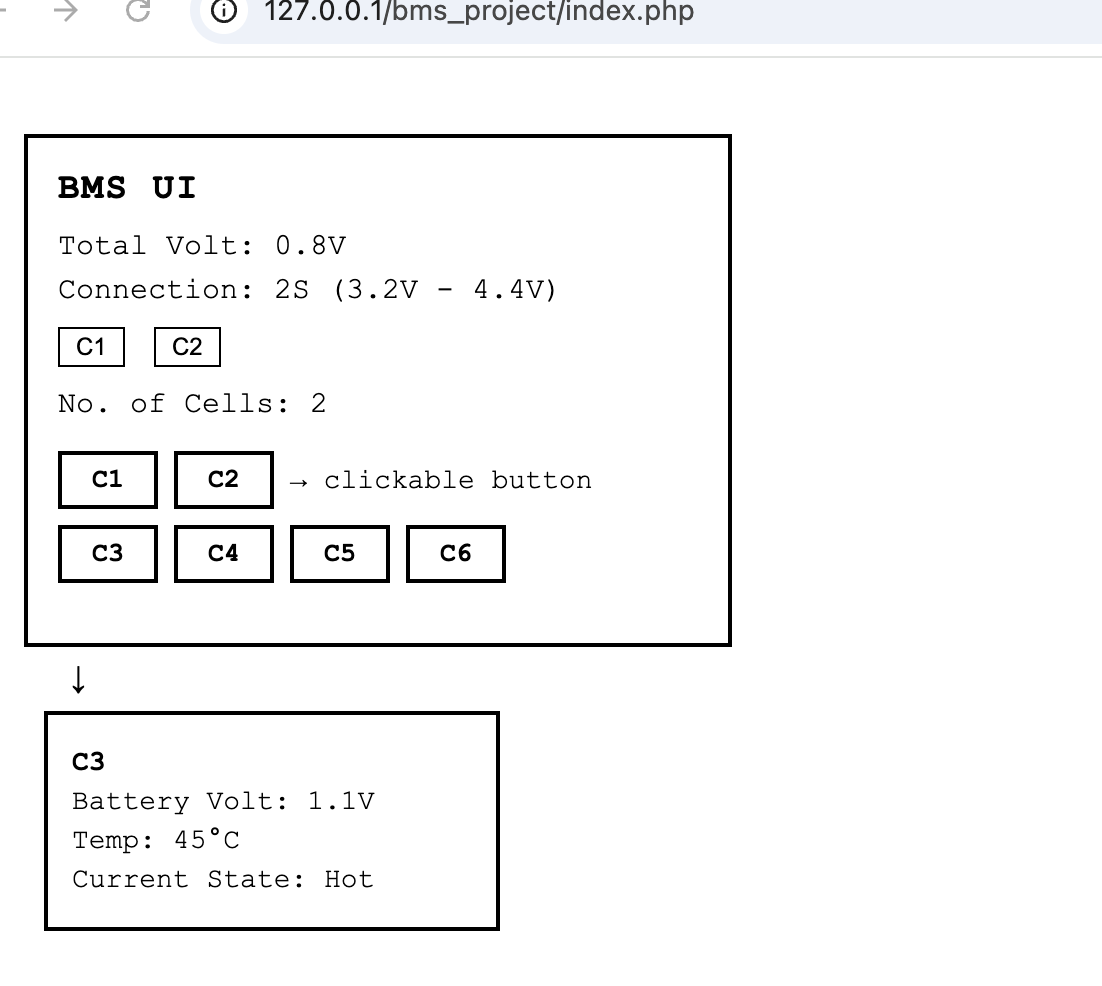
\includegraphics[width=0.70\textwidth]{BMS_BUTTON2.png}

\caption{BMS Button User Interface}

\end{figure}

%%%%%%%%%%%%%%%%%%%%%%%%%%%%%%%%%%%%%%%%%%%%%%%%%%%

\section{Observations}

\begin{itemize}

\item Button controls responded correctly when clicked.

\item The selected battery cell information was displayed successfully.

\item Voltage, temperature, and status were updated dynamically.

\item The graphical interface was simple and easy to operate.

\end{itemize}

%%%%%%%%%%%%%%%%%%%%%%%%%%%%%%%%%%%%%%%%%%%%%%%%%%%

\section{Result}

The BMS button interface was successfully designed and implemented. Each button displayed the corresponding battery-cell information correctly.

%%%%%%%%%%%%%%%%%%%%%%%%%%%%%%%%%%%%%%%%%%%%%%%%%%%

\section{Conclusion}

The experiment demonstrated the implementation of an interactive Battery Management System (BMS) user interface using HTML, CSS, and JavaScript. Button controls effectively displayed battery information, making the interface simple, responsive, and user-friendly.

\newpage

%%%%%%%%%%%%%%%%%%%%%%%%%%%%%%%%%%%%%%%%%%%%%%%%%%%
% REFERENCES
%%%%%%%%%%%%%%%%%%%%%%%%%%%%%%%%%%%%%%%%%%%%%%%%%%%
\begin{thebibliography}{99}

\bibitem{arduino}
Arduino,
\textit{Arduino Uno Rev3},
Arduino Documentation.
Available:
\url{https://docs.arduino.cc/hardware/uno-rev3/}
Accessed: May 26, 2026.

\bibitem{arduinoide}
Arduino,
\textit{Arduino IDE Documentation}.
Available:
\url{https://docs.arduino.cc/software/ide/}
Accessed: May 28, 2026.

\bibitem{sevensegment}
Arduino,
\textit{Seven Segment Display Tutorials and Examples}.
Available:
\url{https://docs.arduino.cc/}
Accessed: June 01, 2026.

\bibitem{ledmatrix}
Arduino,
\textit{LED Matrix Display Documentation}.
Available:
\url{https://docs.arduino.cc/}
Accessed: June 05, 2026.

\bibitem{555}
Texas Instruments,
\textit{NE555 Precision Timer Datasheet}.
Available:
\url{https://www.ti.com/product/NE555}
Accessed: June 20, 2026.

\bibitem{lm741}
Texas Instruments,
\textit{LM741 Operational Amplifier Datasheet}.
Available:
\url{https://www.ti.com/product/LM741}
Accessed: June 28, 2026.

\bibitem{opamp}
Analog Devices,
\textit{Operational Amplifier Technical Articles}.
Available:
\url{https://www.analog.com/en/resources/technical-articles.html}
Accessed: June 30, 2026.

\bibitem{mysql}
Oracle Corporation,
\textit{MySQL Documentation}.
Available:
\url{https://dev.mysql.com/doc/}
Accessed: July 03, 2026.

\bibitem{gfgphp}
GeeksforGeeks,
\textit{PHP MySQL CRUD Operations}.
Available:
\url{https://www.geeksforgeeks.org/php-mysql-crud-operations/}
Accessed: July 05, 2026.

\bibitem{gfghtml}
GeeksforGeeks,
\textit{HTML Button Tag}.
Available:
\url{https://www.geeksforgeeks.org/html-button-tag/}
Accessed: July 08, 2026.

\bibitem{javascript}
MDN Web Docs,
\textit{JavaScript Guide}.
Available:
\url{https://developer.mozilla.org/en-US/docs/Web/JavaScript/Guide}
Accessed: July 09, 2026.

\bibitem{github}
\textsc{GitHub Repository,}
\textit{Source Code Repository for Internship Projects}.
Available:
\url{https://github.com/kittusharma2553-design/2026_GIPEDI_KARUNA_SHARMA.git}
Accessed: July 10, 2026.

\end{thebibliography}
%%%%%%%%%%%%%%%%%%%%%%%%%%%%%%%%%%%%%%%%%%%%%%%%%%%

\end{document}

